\begin{figure}[h]
    \centering
    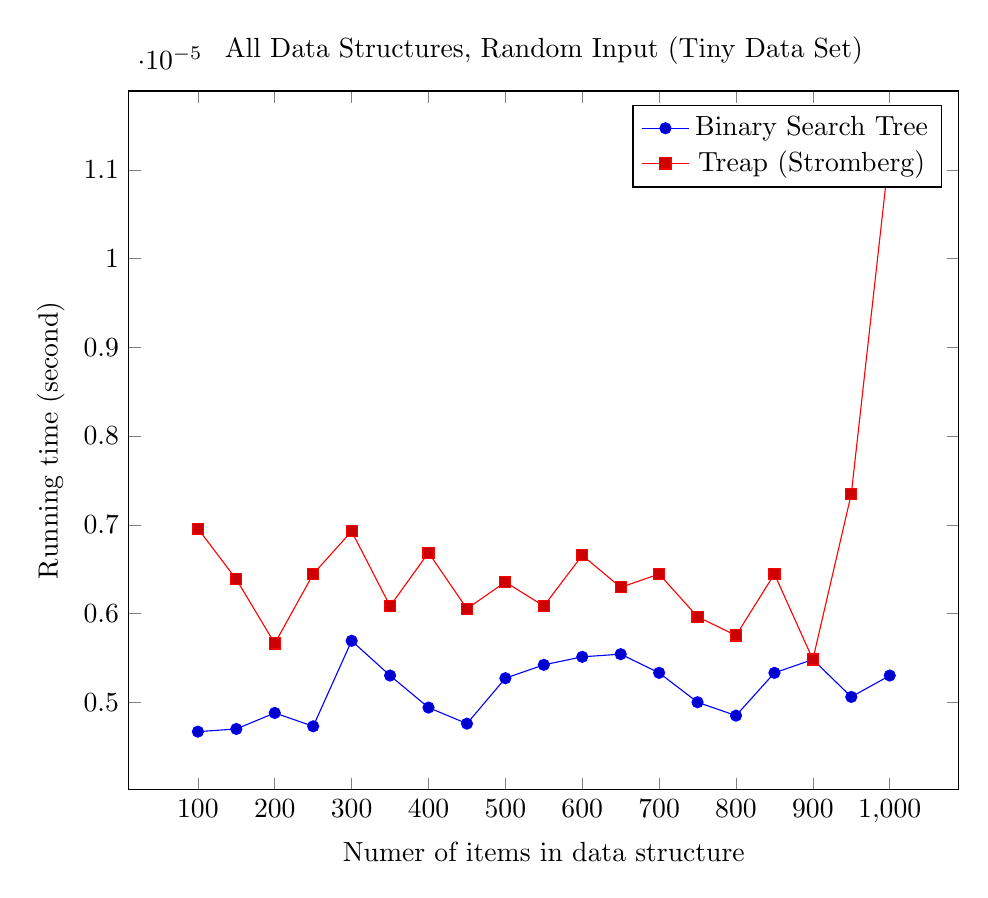
\begin{tikzpicture}
        \begin{axis}[
            xlabel={Numer of items in data structure},
            ylabel={Running time (second)},
            title={All Data Structures, Random Input (Tiny Data Set)},
            width=\textwidth
        ]
		\addplot coordinates {
			(100, 4.668217719627776e-06)
			(150, 4.698335253339181e-06)
			(200, 4.8790404553411545e-06)
			(250, 4.728452786961768e-06)
			(300, 5.692213864616491e-06)
			(350, 5.30068592685673e-06)
			(400, 4.939275522763964e-06)
			(450, 4.758570320673172e-06)
			(500, 5.2705683931453254e-06)
			(550, 5.421156061524712e-06)
			(600, 5.511508662570108e-06)
			(650, 5.541626196237104e-06)
			(700, 5.330803460479317e-06)
			(750, 4.999510590097955e-06)
			(800, 4.848922921674159e-06)
			(850, 5.330803460523726e-06)
			(900, 5.481391128903112e-06)
			(950, 5.059745657431947e-06)
			(1000, 5.300685926812321e-06)
		};
		\addplot coordinates {
			(100, 6.95715027898558e-06)
			(150, 6.3849171391350264e-06)
			(200, 5.6620963309494956e-06)
			(250, 6.445152206513427e-06)
			(300, 6.927032745274176e-06)
			(350, 6.0837418023762526e-06)
			(400, 6.686092475893801e-06)
			(450, 6.0536242687092566e-06)
			(500, 6.354799605468031e-06)
			(550, 6.0837418023762526e-06)
			(600, 6.655974942226805e-06)
			(650, 6.294564538089631e-06)
			(700, 6.445152206513427e-06)
			(750, 5.963271667663861e-06)
			(800, 5.752448931950483e-06)
			(850, 6.4451522064690184e-06)
			(900, 5.481391128903112e-06)
			(950, 7.348678216745341e-06)
			(1000, 1.1233840060809187e-05)
		};
        \legend{Binary Search Tree, Treap (Stromberg)}
        \end{axis}
    \end{tikzpicture}
    \caption{Average of 10 operations, benchmarked every 50, starting at 100.}
\end{figure}